\section{Lecture 7}

\subsection{Revisiting Exponential}

\begin{definition}
    Let $z \in \Cbb$, we define the complex exponential map $e^z: \Cbb \to \Cbb$ as
    \[e^z \coloneqq 1 + z + \frac{z^2}{2!} + ... = \sum_{n = 0}^\infty \frac{z^n}{n!}\]
\end{definition}

\begin{theorem}[Euler's Identity]
Let $x \in \Rbb$, then
\[e^{ix} = cos(x) + i sin(x)\]
\end{theorem}

\begin{proof}
We can show this via explicit computation, indeed,
\begin{align*}
    e^{ix} &= \sum_{n = 0}^\infty \frac{(ix)^n}{n!}\\
    &= \sum_{k = 0}^\infty (-1)^k \frac{x^{2k}}{(2k)!} + i \sum_{k = 0} (-1)^k \frac{x^{2k + 1}}{(2k + 1)!} \tag*{Separate even and odd degree terms}\\
    &= cos(x) + i sin(x) \tag*{Taylor Series}
\end{align*}
\end{proof}

\begin{lemma}\label{lem::real_analy_fact}
Facts from Analysis:
\begin{enumerate}
    \item For every $r \in \Rbb$, $\sum_{n = 0}^\infty \frac{r^n}{n!}$ converges absolutely
    \item If $a_n \in \Cbb$ and $\sum_{n = 0}^\infty |a_n|$ converges, then $\sum_{n = 0}^\infty a_n$ converges
    \item If $L_a = \sum_{n = 0}^\infty a_n, L_b = \sum_{m = 0}^\infty b_m$ converges absolutely, then
    \[\sum_{n = 0}^\infty \sum_{k = 0}^n a_k b_{n - k}\]
    converges to
    \[(\sum_{n = 0}^\infty a_n) \cdot (\sum_{m = 0}^\infty b_m)\]
\end{enumerate}
This will helpful in proving some identities.
\end{lemma}

\begin{proof}
For $(1)$, we will use the ratio test. Indeed, consider $a_n = \frac{r^n}{n!}$, then
\[\lim_{n \to \infty} |\frac{a_{n+1}}{a_n}| = \lim_{n \to \infty} |\frac{r}{n + 1}| = 0 < 1\]
Thus, the series converges absolutely.\\\\
For $(2)$, let $b_n = \sum_{i = 1}^n a_i, c_n = \sum_{i = 1}^n |a_i|$. We note that the topology $\Cbb$ is homeomorphic to the Euclidean topology on $\Rbb^2$, so in particular $\Cbb$ is a complete metric space, so a sequence is convergent if and only if it is Cauchy. We know $c_n$ converges, so for every $\epsilon > 0$, there exists some $N_c$ such that for all $i, j > N_c$.
\[|c_i - c_j| < \epsilon\]
It remains for us to show that $b_n$ is also Cauchy. Indeed, if $i = j$, then we are done. Without loss, we will then assume $j > i$, then
\begin{align*}
    |b_i - b_j| &= |\sum_{k = i + 1}^j a_k|\\
    &\leq \sum_{k = i + 1}^j |a_k| \tag*{Triangle's Inequality}\\
    &= |c_i - c_j|\\
    &< \epsilon
\end{align*}
Thus, $\{b_n\}$ is Cauchy and converges.\\\\
For $(3)$, $(\sum_{n = 0}^\infty a_n) \cdot (\sum_{m = 0}^\infty b_m)$ certainly converges to $L_a \cdot L_b$. Now write $(\sum_{n = 0}^\infty a_n) \cdot (\sum_{m = 0}^\infty b_m) = \sum_{n = 0}^\infty \sum_{m = 0}^\infty a_n b_m$, this corresponds exactly to the terms of $\sum_{n = 0}^\infty \sum_{k = 0}^n a_k b_{n - k}$. The exact combinatorics is left as details to the reader.
\end{proof}

\begin{corollary}
Let $e^z$ be the complex exponential map, then
\begin{itemize}
    \item $e^z$ converges for all $z \in \Cbb$
    \item $e^{z + w} = e^z \cdot e^w$ for all $z, w \in \Cbb$
\end{itemize}
\end{corollary}

\begin{proof}
For the first, let $a_n = \sum_{k = 1}^n |\frac{z^k}{k!}|$. It suffices for us to prove that $a_n$ converges as absolute convergence implies monotone convergence from Lemma~\ref{lem::real_analy_fact}(2). But we note that 
\[|\frac{z^k}{k!}| = \frac{|z|^k}{k!}\]
and $|z|$ is a real number, so Lemma~\ref{lem::real_analy_fact}(1) tells us that $a_n$ converges.\\\\
For the second, we note that
\begin{align*}
    e^{z + w} &= \sum_{n = 0}^\infty \frac{(z + w)^n}{n!}\\
    &= \sum_{n = 0}^\infty \sum_{k = 0}^n {n \choose k} \frac{z^k w^{n-k}}{n!} \tag*{Binomial Theorem}\\
    &= \sum_{n = 0}^\infty \sum_{k = 0}^n \frac{z^k}{k!} \frac{w^{n-k}}{(n - k)!}\\
    &= (\sum_{n = 0}^\infty \frac{(z)^n}{n!}) \cdot (\sum_{n = 0}^\infty \frac{(w)^n}{n!}) \tag*{By Lemma~\ref{lem::real_analy_fact}(3)}\\
    &= e^z \cdot e^w
\end{align*}
\end{proof}

\begin{proposition}
We can also recover $\cos(z)$ and $\sin(z)$ from $e^z$ as
\[\cos(z) = \frac{e^{iz} + e^{-iz}}{2}, \sin(z) = \frac{e^{iz} - e^{-iz}}{2i}\]
If $x \in \Rbb$, we also have that
\[\cos(x) = \Re e^{ix}, \sin(x) = \Im e^{ix}\]
\end{proposition}

\subsection{Complex Logarithms}

As in the case of $\Rbb$, we want to define $\log(z)$ as an inverse to $e^z$ such that
\[e^{\log(z)} = z\]
The problem is that $e^z$ is not actually injective, so there are multiple choices for $\log(z)$. Consequently, this will result in $\log(z)$ not being continuous on all of $\Cbb$.

\begin{question}
Given $z$, can we find all solutions satifying $e^w = z$?
\end{question}

\begin{proof}[Answer]
We will again leverage on Polar Coordinates. Indeed, write $z = re^{i \theta}, w = x + iy$, then we have that
\[r e^{i \theta} = e^{x + iy} = e^{x} e^{iy}\]
Thus, $x = \log(r), y = \theta + 2 \pi k$.\\\\
Thus, $w$ is of the form $w_k = \log(r) + i(\theta + 2 \pi k)$
\end{proof}

\begin{definition}[Complex Logarithm]
    For $z \in \Cbb \setminus \{0\}$, write $z = re^{i \theta}, \theta \in [-\pi, \pi]$. Then we define
    \[\log(z) = \log(r e^{i \theta}) \coloneqq \log(r) + i \theta\]
    $\theta$ is sometimes refered to as the \textbf{principal argument} of $z$ and we denote $Arg(z) = \theta$.
\end{definition}

\begin{remark}
Note that the complex logarithm $\log(z)$ is not continuous on all of $\Cbb$:
\[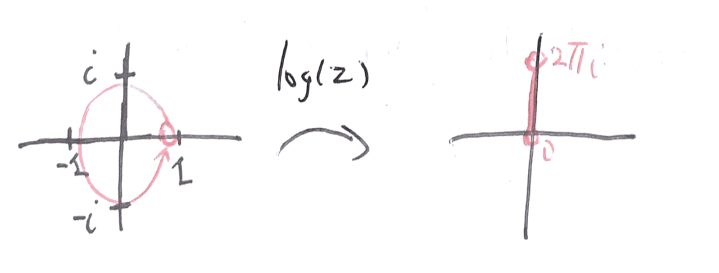
\includegraphics[width=0.5\textwidth]{Figures/complex_log.png}\]
As you trace around the unit circle, going back to $z = 1$ presents a problem.\\\\
Therefore, we can only define the complex logarithm up to a \textbf{branch cut} that's a radial line extending out from the origin. We will without loss choose this branch to be $(-\infty, 0]$
\end{remark}

\begin{proposition}
$\log(z)$ is holomorphic on $\Cbb \setminus (-\infty, 0]$ and in fact $\frac{d}{dz} \log(w) = \frac{1}{w}$
\end{proposition}

\begin{proof}
One way to do this is to use the Cauchy-Riemann equations in polar coordinates. We will however use the Inverse Function Theorem instead. Indeed, we note that on $\Cbb \setminus (-\infty, 0]$, $z \mapsto e^z$, when viewed as a function from $\Rbb^2$ to $\Rbb^2$, is a smooth function whose derivative is exactly
\[(e^z)' = e^x \begin{pmatrix} cos(y) & -sin(y)\\ sin(y) & cos(y) \end{pmatrix}\]
, which satisfies the matrix representation of complex numbers (hence we can extend the argument to holomorphic functions). Thus, the inverse function theorem tells us that $g(z) = \log(z)$ is also holomorphic and that
\[g'(f(x)) = (f'(x))^{-1}\]
This equation tells us that, locally for all $w = e^z \in \Cbb \setminus (-\infty, 0]$,
\[\frac{d}{dz} \log(w) = e^{-x}\begin{pmatrix} cos(y) & sin(y)\\ -sin(y) & cos(y) \end{pmatrix} = (e^{z})^{-1} = \frac{1}{w}\]
Note that the branch cut does not prevent the existence of a local inverse, but it does prevent the existence of a global inverse on all of $\Cbb$.
\end{proof}

\begin{remark}
Let $z \in \Cbb \setminus (-\infty, 0]$, then since $\frac{1}{z}$ is primitive on the path $1$ to $z$, we have that:
\[\int_1^z \frac{d\xi}{\xi} = \log(z) - \log(1) = \log(z)\]
\end{remark}

\subsection{Homotopy Invariance of Integral}

Let $f \in Hol(\Omega)$ and $\gamma: [a, b] \to \Gamma$ is continous and $\Gamma \subset \Omega$, then we can define the integral
\[\int_\gamma f(z) dz\]

Informally, we can define this because at each point on $\gamma$, we can find some disk to represent $f$ as a power series with a primitive $F$, then we can split $[a, b]$ into a union of (not necessarily uniform) subintervals, then the integral $\gamma$ can be approximated as a sum of the anti-derivatives $F_k$ at each end-points.

We can formally justify this with what's called the Lebesgue's Number Lemma.

\begin{lemma}[Lebesgue's Number Lemma]
Let $K$ be a compact metric space and let $\{U_a\}$ be an open cover for $K$, then there exists some $\delta > 0$ (we call the \textbf{Lebesgue Number}) such that for all $x \in K$, there exists some $a$ such that $B_{x, \delta} \subset U_a$
\end{lemma}

\begin{proof}
For all $x \in K$, since $\{U_a\}$ is an open cover of $K$, there exists some $a$ such that $x \in U_a$. Since $U_a$ is open, there exists some $r(x) > 0$ small enough such that $B_{x, 2r(x)} \subset U_\alpha$.\\\\
Note that $\{B_{x, r(x)}\}$ running over all $x \in K$ is an open cover of $K$. Since $K$ is compact, we in fact have a finite subcover:
\[B_{x_1, r_1}, ..., B_{x_n, r_n}\]
Choose $\delta = \min \{r_i\}$. Now for all $x \in K$, it belongs to one of the $B_{x_k, r_k} \subset U_a$.\\\
Then we claim $x \in B_{x, \delta} \subset B_{x_k, 2r_k} \subset U_a$. To do this, we need to verify $B_{x, \delta} \subset B_{x_k, 2r_k}$. Indeed, for all $y \in B_{x, \delta}$, we have that
\[d(y, x_k) \leq d(y, x) + d(x, x_k) < \delta + r_k \leq 2r_k\]
This concludes the proof.
\end{proof}

To apply this lemma in our context, we take $K = [a, b]$ and for all $s \in [a, b]$, we define $U_s = \gamma^{-1}(D_{\gamma(s), r(s)})$, where $r(s)$ is the radius of convergence of $\gamma(s)$ under the power-series. Then we can apply the Lebesgue's Number Lemma.

\begin{question}
Is the integral well-defined up to two different splitting?
\end{question}

\begin{proof}[Answer]
Yes, the idea is that given two splitting on the interval, one can join them using a refinement by taking smaller intervaks of both of them and used the associated anti-derivative from either original splittings. To be more rigorous, let $\{I_k\}$ and $\{J_n\}$ be two different splittings of the interval $[0, 1]$. Now define
\[I_{k, n} \coloneqq I_k \cap J_n\]
Then we note that, by definition, the integral over the splitting $I_{k, n}$ would be of the form
\begin{align*}
    \sum \int_{I_{k, n}} f(z) dz &= \sum_{k} \sum_{n} \int_{I_{k, n}} f(z) dz\\
    &= \sum_k [\sum_{n} \int_{I_{k, n}} f(z) dz]\\
    &= \sum_k \int_{I_k} f(z) dz
\end{align*}
Similarly, we can also show that
\[\sum \int_{I_{k, n}} f(z) dz = \sum_n \int_{J_n} f(z) dz\]
Thus, the two splittings yield the same integral.
\end{proof}

\begin{definition}
    Let $\gamma_0, \gamma_1: [a, b] \to \Omega$ be continuous. We say $\gamma_0$ is \textbf{homotopy equivalent} to $\gamma_1$ if there exists a continuous function $\Gamma: [a, b] \times [0, 1] \to \Omega$ such that $\Gamma(s, 0) = \gamma_0(s)$ and $\gamma(s, 1) = \gamma_1(s)$ for all $s \in [a, b]$.\\
    We will also assume that either:
        \begin{itemize}
            \item All pathes are closed, for all $t$
            \[\Gamma(a, t) = \Gamma(b, t)\]
            \item OR Endpoints are fixed
            \[\Gamma(a, t) = \gamma_0(a) = \gamma_1(b)\]
            \[\Gamma(b, t) = \gamma_0(b) = \gamma_1(b)\]
        \end{itemize}
\end{definition}

\begin{theorem}
If $\gamma_0, \gamma_1$ are homotopy equivalent in $\Omega$ and $f \in Hol(\Omega)$, then
\[\int_{\gamma_0} f(z) dz = \int_{\gamma_1} f(z) dz\]
\end{theorem}

\begin{remark}
In a simply connected domain, any two pathes are homotopy equivalent. In otherwords, the path of integration is irrelevant.
\end{remark}